\documentclass[a4paper,class=article,border=10pt,tikz]{standalone}

%mypackages
\usepackage{pythontex}
\usepackage{pgfplots}
\usepackage{amsmath}
\usepackage{titlesec}
\usepackage{tikz}
\usetikzlibrary{shapes.geometric}
\usetikzlibrary{positioning}
\usetikzlibrary{snakes,calc,positioning,patterns,angles,quotes,decorations.pathmorphing,decorations.markings}
% \titleformat{<command>}[<shape>]{<format>}{<label>}{<sep>}{<before-code>}[<after-code>]
%\titleformat{\section}{\normalfont\Large\bfseries}{\thesection.}{10pt}{}
% \titlespacing{<command>}{<left>}{<before-sep>}{<after-sep>}
%\titlespacing{\section}{0pt}{14pt}{7pt}

%\titleformat{\subsection}{\normalfont\itshape}{\thesubsection.}{10pt}{}
%\titlespacing{\subsection}{0pt}{12pt}{6pt}
% set font encoding for PDFLaTeX, XeLaTeX, or LuaTeX
\usepackage{ifxetex,ifluatex}
\if\ifxetex T\else\ifluatex T\else F\fi\fi T%
  \usepackage{fontspec}
\else
  \usepackage[T1]{fontenc}
  \usepackage[utf8]{inputenc}
  \usepackage{lmodern}
\fi

\usepackage{hyperref}


\title{Title of Document}
\author{Name of Author}

% Enable SageTeX to run SageMath code right inside this LaTeX file.
% http://doc.sagemath.org/html/en/tutorial/sagetex.html
% \usepackage{sagetex}

% Enable PythonTeX to run Python – https://ctan.org/pkg/pythontex
% \usepackage{pythontex}

\begin{document}

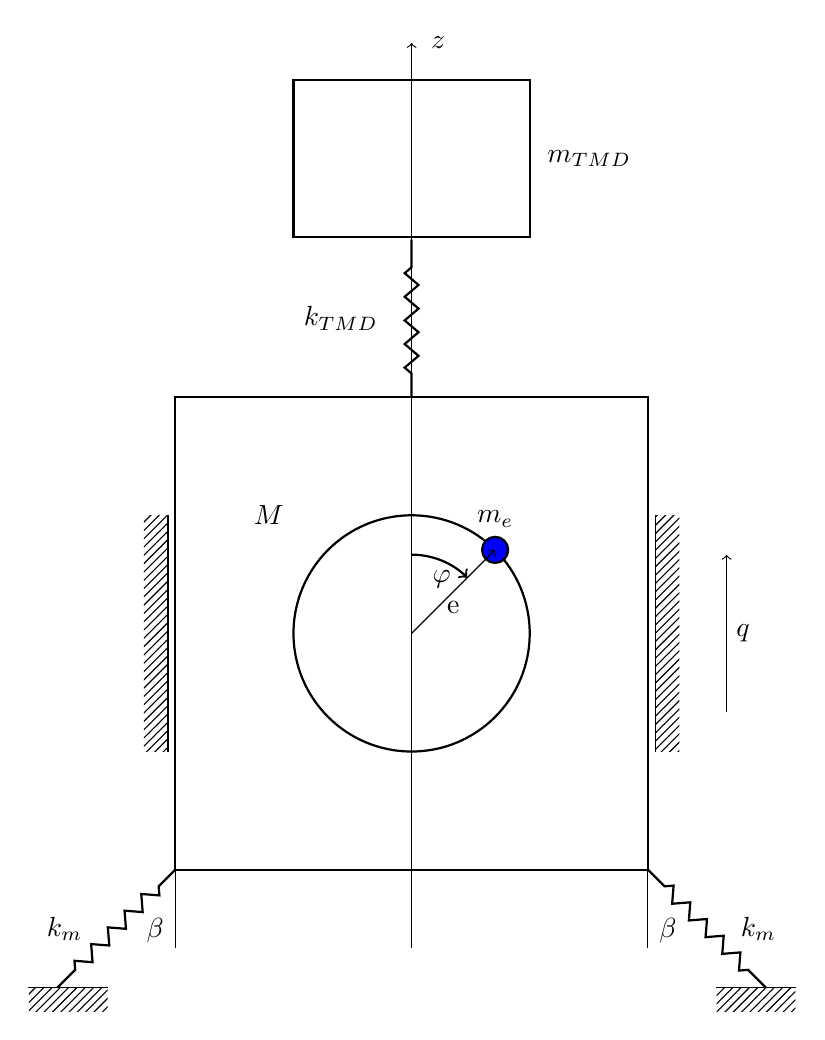
\begin{tikzpicture}[scale=1, transform shape]
 \coordinate (origo) at (0,0);

\tikzstyle{spring}=[thick,decorate,decoration={zigzag,pre length=0.3cm,post length=0.3cm,segment length=0.3cm}]

\tikzstyle{damper}=[thick,decoration={markings,  
  mark connection node=dmp,
  mark=at position 0.5 with 
  {
    \node (dmp) [thick,inner sep=0pt,transform shape,rotate=-90,minimum width=15pt,minimum height=3pt,draw=none] {};
    \draw [thick] ($(dmp.north east)+(2pt,0)$) -- (dmp.south east) -- (dmp.south west) -- ($(dmp.north west)+(2pt,0)$);
    \draw [thick] ($(dmp.north)+(0,-5pt)$) -- ($(dmp.north)+(0,5pt)$);
  }
}, decorate]

\tikzstyle{ground}=[fill,pattern=north east lines,draw=none,minimum width=0.75cm,minimum height=0.3cm]



   %draw axes
    %\fill[black] (origo) circle (0.05);

    
    \node (M) [draw,outer sep=0pt,thick,minimum width=6cm, minimum height=6cm,yshift=2cm,label={left,xshift=1.5cm,yshift=1.5cm:$M$}] at (origo) {};
    %\node (m1_label) at ($(M)+(0:0.5cm)$) {$m$};

    \draw [spring] (M.south west)  node[] (left_spring){}  --++ (-1.5cm,-1.5cm) node[midway,left,xshift=-0.3cm] {$k_{m}$};
    
\draw [spring] (M.south east)  node[] (right_spring){}  --++ (1.5cm,-1.5cm) node[midway,right,xshift=0.3cm] {$k_{m}$};
\node (R) [draw,circle,outer sep=0pt,thick, minimum height=3cm] at (M.center) {};
%\node (me) [fill=blue,draw,circle,outer sep=0pt,thick, minimum height=0.001cm] at (45:1.25) {};
\node (me) [fill=blue,draw,circle,outer sep=0pt,thick, minimum height=0.001cm,label={above:$m_{e}$}] at (R.north east) {};
    %\fill [black] (M.center) circle (0.05);
\draw[thick, ->,] (M)[xshift=0cm,yshift=1.0cm ] arc (90:45:1.0cm) node[below,midway,xshift=-0.0cm,yshift=0.0cm] {$\varphi$};

   % \node (beam) [fill=gray,anchor=north,xshift=0cm,yshift=0cm,minimum width=2cm,minimum height=0.05pt] at (origo) {} node[right]{$m_{beam}=0$};

%     \draw [ultra thick] (k_sup_spring_left.west) -- (k_sup_spring_right.east) node[midway] (beam_center) {};
    
    
%         \node (road_sur) [fill=black,anchor=north,xshift=0cm,yshift=-2cm,minimum width=2cm,minimum height=0.05cm] at (beam) {};

%beam_center.center

\node (ground1) [ground,anchor=north west,xshift=-0.25cm,yshift=-0cm,minimum width=1cm] at (left_spring.east)[xshift=-1.75cm,yshift=-1.5cm] {};

\node (ground2) [ground,anchor=north east,xshift=0.25cm,yshift=-0cm,minimum width=1cm] at (right_spring.east)[xshift=1.5cm,yshift=-1.5cm] {};
\draw (ground1.north west) --(ground1.north east);
\draw (ground2.north west) --(ground2.north east);
\draw[->,transform canvas={xshift=4cm,yshift=1cm}] (origo)--++(0,2cm) node[label={right,midway:$q$}] {};
\draw[thin] (M.south east) --++(0,-1cm) node[above,label={right,above,xshift=-0.1cm,yshift=0.1cm:$\beta$}] {};
\draw[thin] (M.south west) --++(0,-1cm) node[above,label={left,above,xshift=0.1cm,yshift=0.1cm:$\beta$}] {};
\draw[->](0,-2cm)--(0,9.5cm) node[label={right:$z$}] {};

\node (wall1) [ground,anchor=center,xshift=0cm,yshift=-0cm,minimum width=3cm,rotate=90] at (M.east)[yshift=-0.25cm] {};
\node (wall2) [ground,anchor=center,xshift=-0.25cm,yshift=-0cm,minimum width=3cm,rotate=-90] at (M.west)[xshift=0cm,yshift=0cm] {};
\draw (wall1.north west) --(wall1.north east);
\draw (wall2.north west) --(wall2.north east);
\draw[->] (M.center)--(me.center) node[below,midway]{e};
\draw [spring] (M.north)  node[] (center_spring){}  --++ (0cm,2cm) node[midway,left,xshift=-0.3cm] {$k_{TMD}$};
\node (mass) [draw,outer sep=0pt,thick,minimum width=3cm, minimum height=2cm, label={right,xshift=0.1cm:$m_{TMD}$}] at (center_spring.north)[yshift=2.9cm] {};
\end{tikzpicture}

\end{document}
